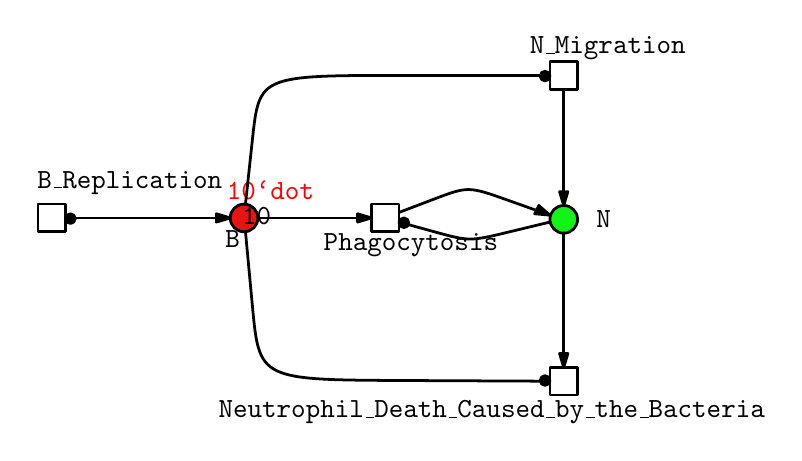
\begin{tikzpicture}[x=0.5pt,y=-0.5pt]

\definecolor{BLACK}{RGB}{0,0,0}
\definecolor{r232g19b19}{RGB}{232,19,19}
\draw[BLACK, solid, line join=round, line cap=round, line width=1, fill=r232g19b19]
	(199,143) ellipse[x radius=10, y radius=10];
\draw[BLACK]
	(179,158.5) node[rotate=0, font=\ttfamily\normalsize, BLACK, right=-.25]
	{B};
\draw[BLACK]
	(191,141.5) node[rotate=0, font=\ttfamily\normalsize, BLACK, right=-.25]
	{10};
\definecolor{RED}{RGB}{255,0,0}
\draw[BLACK]
	(180,123.5) node[rotate=0, font=\ttfamily\normalsize, RED, right=-.25]
	{10`dot};
\definecolor{r18g244b21}{RGB}{18,244,21}
\draw[BLACK, solid, line join=round, line cap=round, line width=1, fill=r18g244b21]
	(430,144) ellipse[x radius=10, y radius=10];
\draw[BLACK]
	(447,143.5) node[rotate=0, font=\ttfamily\normalsize, BLACK, right=-.25]
	{N};
\definecolor{WHITE}{RGB}{255,255,255}
\draw[BLACK, solid, line join=round, line cap=round, line width=1, fill=WHITE]
	(50,133) rectangle +(20,20);
\draw[BLACK]
	(43,117.5) node[rotate=0, font=\ttfamily\normalsize, BLACK, right=-.25]
	{B\_Replication};
\draw[BLACK, solid, line join=round, line cap=round, line width=1, fill=WHITE]
	(291,133) rectangle +(20,20);
\draw[BLACK]
	(250,162.5) node[rotate=0, font=\ttfamily\normalsize, BLACK, right=-.25]
	{Phagocytosis};
\draw[BLACK, solid, line join=round, line cap=round, line width=1, fill=WHITE]
	(420,251) rectangle +(20,20);
\draw[BLACK]
	(174,283.5) node[rotate=0, font=\ttfamily\normalsize, BLACK, right=-.25]
	{Neutrophil\_Death\_Caused\_by\_the\_Bacteria};
\draw[BLACK, solid, line join=round, line cap=round, line width=1, fill=WHITE]
	(420,30) rectangle +(20,20);
\draw[BLACK]
	(399,20.5) node[rotate=0, font=\ttfamily\normalsize, BLACK, right=-.25]
	{N\_Migration};
\draw[BLACK, solid, line join=round, line cap=round, line width=1]
	(70,143) -- (189,143);
\draw[BLACK, solid, line join=round, line cap=round, line width=1, fill=BLACK]
	(189,143) -- (179,146) -- (179,140) -- (189,143) -- cycle;
\draw[BLACK, solid, line join=round, line cap=round, line width=1]
	(209,143) -- (291,143);
\draw[BLACK, solid, line join=round, line cap=round, line width=1, fill=BLACK]
	(291,143) -- (281,146) -- (281,140) -- (291,143) -- cycle;
\draw[BLACK, solid, line join=round, line cap=round, line width=1]
	(430,154) -- (430,251);
\draw[BLACK, solid, line join=round, line cap=round, line width=1, fill=BLACK]
	(430,251) -- (427,241) -- (433,241) -- (430,251) -- cycle;
\draw[BLACK, solid, line join=round, line cap=round, line width=1]
	(430,50) -- (430,134);
\draw[BLACK, solid, line join=round, line cap=round, line width=1, fill=BLACK]
	(430,134) -- (427,124) -- (433,124) -- (430,134) -- cycle;
\draw[BLACK, solid, line join=round, line cap=round, line width=1]
	(189,143) -- (70,143);
\draw[BLACK, solid, line join=round, line cap=round, line width=1, fill=BLACK]
	(73.5,143.5) ellipse[x radius=3.5, y radius=3.5];
\draw[BLACK, solid, line join=round, line cap=round, line width=1]
	(200,153) -- (205,206.5) .. controls (210,260) .. (315,260.5) -- (420,261);
\draw[BLACK, solid, line join=round, line cap=round, line width=1, fill=BLACK]
	(416.5,260.5) ellipse[x radius=3.5, y radius=3.5];
\draw[BLACK, solid, line join=round, line cap=round, line width=1]
	(200,133) -- (205,86.5) .. controls (210,40) .. (315,40) -- (420,40);
\draw[BLACK, solid, line join=round, line cap=round, line width=1, fill=BLACK]
	(416.5,40.5) ellipse[x radius=3.5, y radius=3.5];
\draw[BLACK, solid, line join=round, line cap=round, line width=1]
	(311,139) -- (336,129.5) .. controls (361,120) .. (390.5,130.5) -- (420,141);
\draw[BLACK, solid, line join=round, line cap=round, line width=1, fill=BLACK]
	(420,141) -- (409,140) -- (412,134) -- (420,141) -- cycle;
\draw[BLACK, solid, line join=round, line cap=round, line width=1]
	(420,146) -- (391,153) .. controls (362,160) .. (336.5,153) -- (311,146);
\draw[BLACK, solid, line join=round, line cap=round, line width=1, fill=BLACK]
	(314.5,146.5) ellipse[x radius=3.5, y radius=3.5];
\end{tikzpicture}